%-----------------------------------------------------
% Chapter: Introduction
%-----------------------------------------------------
\chapter{Introduction}
\label{chap:intro}
\section{Overview}
Both language modelling and text classification are active research areas within natural language processing. The primary goal of language modelling is to provide a probability distribution for sequences of words. Recent neural language models have provided state of the art performance for evaluation tasks such as the Penn Treebank(REF). Text classification, which is the task of classifying text into one or more predefined categories has applications in areas such as sentiment analysis, topic labelling and spam detection.   

\noindent
\newline
Recurrent neural networks have been deployed successfully in both language modelling and text classification tasks. Training these types of networks on textual data involves the conversion of text to vector representations which can  result in either sparse or dense word vectors. Sparse representation of words, such as a one-hot encoding suffer from the curse of dimensionality due to the dimensionality of the word vector growing linearly with the size of the vocabulary. Dense representations of words, also known as word embeddings, offer smaller continuous word representations which are able to encode semantic and syntactic meanings within texts. The utilization of word embeddings has been highly successful in many natural language processing tasks and has found effective usage in downstream machine learning pipelines.

\noindent
\newline
Often accompanying text corpora are associated covariates, e.g. author demographic or publication genre, which provide additional metadata about a corpus. CoVeR (REF), a novel tensor decomposition method for learning covariate specific word embeddings, is an extension of the GloVe algorithm which aims to encode covariate information with learned embeddings.

\section{The Songwriters Dilemma}
Songwriting is an integral part of the song making process which often draws upon past events and experiences. Structure and content both contribute heavily towards the success of a song; with the latter being a key factor on the extent to which a song resonates with a listener. A problem commonly faced by songwriters is that of word choice, through which they can express their ideas clearly and concisely.

\noindent
\newline
In general, skilled writers are attributed with having vast vocabulary ranges. For adults, the average vocabulary ranges between 15,000-23,000 words(REF). Examining his works alone, Shakespeare is said to have had an approximate vocabulary size of 30,000 words (REF) (FOOTNOTE HERE SKEWED). Nonetheless, a skilled songwriters ability to write impactful lyrics is not down to vocabulary size alone, but effective word choice.
 
\noindent
\newline
As shown in a study examining vocabulary range within Hip-Hop, which recently surpassed Rock as the most popular genre in America (REF HERE), more is not always better. The study examines the unique word count of 150 famous Hip-Hop artists across their first 35,000 lyrics. Aesop Rock, ranked 1st on the list, recorded a count of 7,392 unique words across his first 35,000 lyrics. In contrast, rappers Drake and Future, ranked 130th and 131st respectively, had an average unique word count of 3,334 words used across their first 35,000 lyrics; a 55\% decrease from Aesop Rocks count. 
\begin{figure}[h]	
	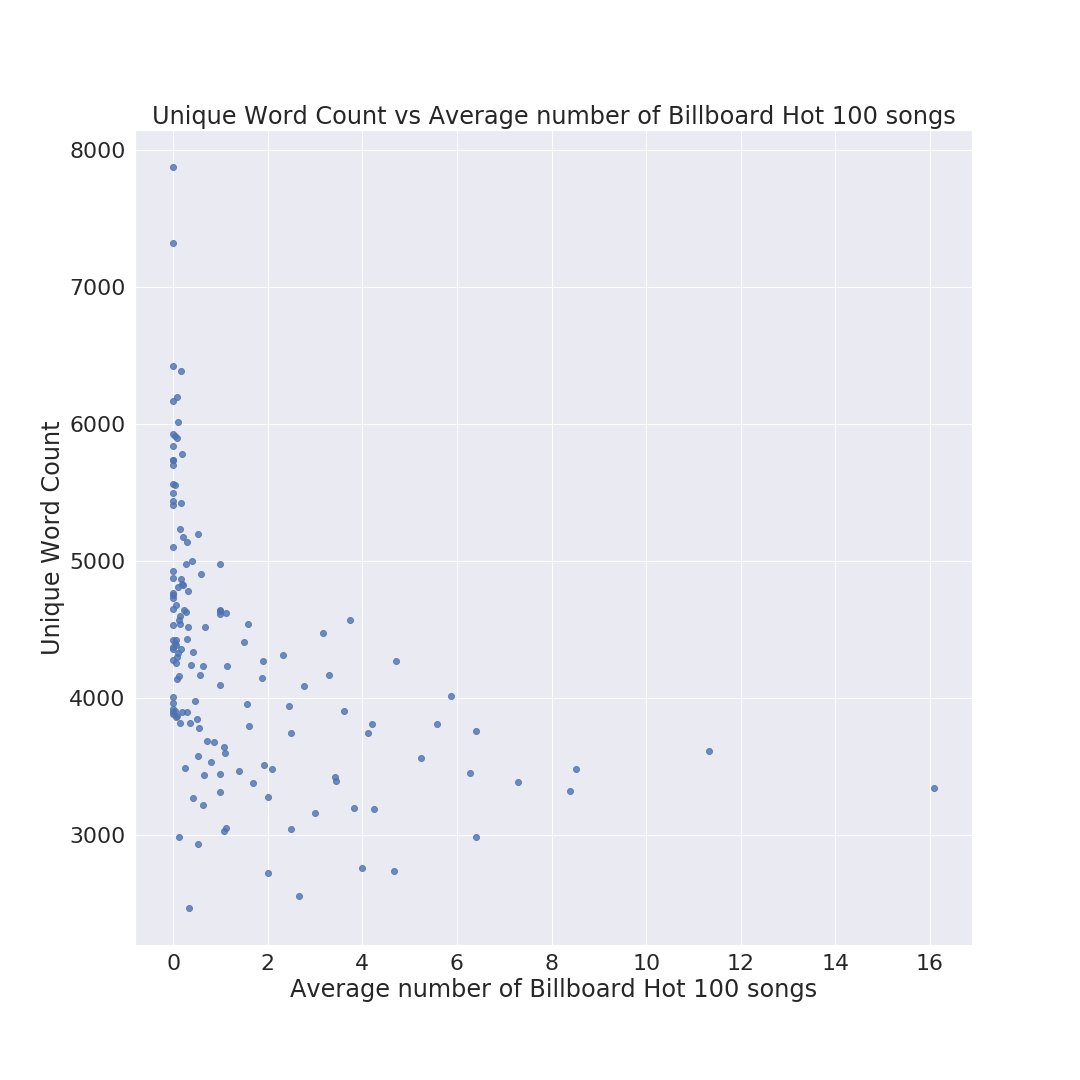
\includegraphics[width=10cm, height=10cm]{./figures/fig1}
	\centering
	\caption{Average number of Billboard 100 songs during artist activity, compared to unique word count across an artists first 35,000 words.}
	\label{fig:fig1}
\end{figure}

\noindent
\newline
To validate the earlier claim that vocabulary range is not indicative of a songwriters ability to write impactful lyrics, the unique word count per artist was compared against the average number of Billboard 100 songs across an artist had across their career. Pearson's Correlation Coefficient , which is used to measure the linear relationship between two variables, was applied to both unique word count and average number of Billboard 100 songs. This resulted in a correlation coefficient of -0.42, indicating a weak inverse correlation between the pairs of data. This value supports the earlier claim that vocabulary range is not indicative of a songwriters ability.

\noindent
\newline
Common methods used to improve songwriting competency include group writing and vocabulary expansion. More recently, software solutions such as MasterWriter(REF) have been used to consolidate previous methods. An inherent problem within software solutions like MasterWriter is the static nature of features such as fixed word and rhyming dictionaries. Consequently, these applications fail to address the ambiguous usage of words resulting from the emerging nature of natural language.

\noindent
\newline
After the completion of song lyrics another secondary problem often faced by less experienced songwriters is choice of instrumental style. 

\section{Goals and Objectives}
\subsection{SONGIFAI - A proposed solution}
The goal of this project is to explore the use of CoVeR derived word embeddings to help with both language modelling and text classification tasks. To contextualise the project aims, both models are applied to a possible use case: a protoype software solution to help reduce common problems faced by songwriters. With this in mind, a prototype solution, SONGIFAI is proposed. SONGIFAI provides two main features namely lyric assistance through predictive text and word suggestions, as well as lyric genre classification. The covariates explored in this project are the following music genres: \textit{Pop}, \textit{Rock} and \textit{Hip-Hop}.
\subsection{High Level Architecture}
\begin{figure}[h]	
	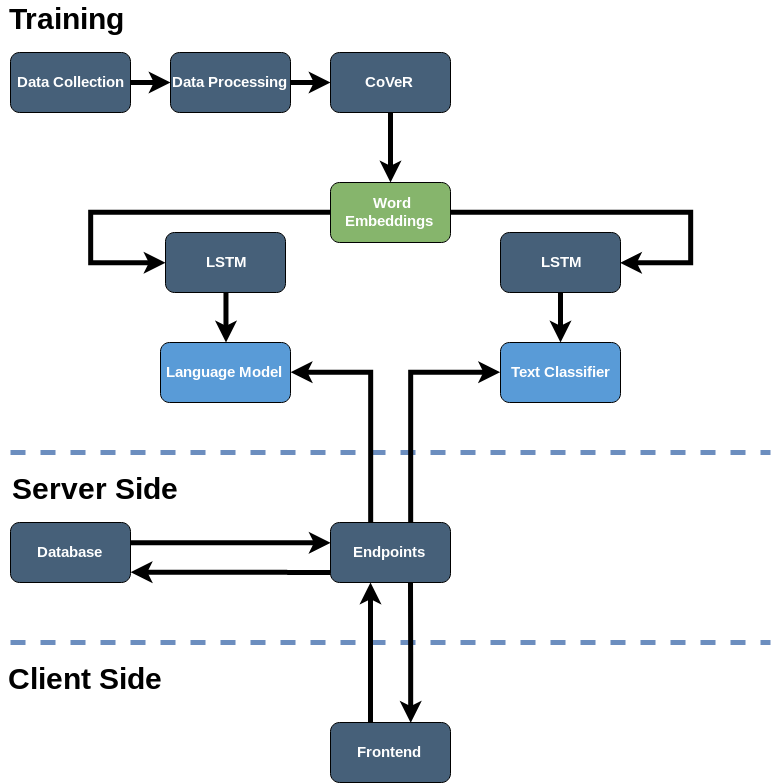
\includegraphics[width=13cm, height=14cm]{./figures/fig7}
	\centering
	\caption{High level architecture for the project}
	\label{fig:fig7}
\end{figure}
